\section{Introduction}

In long-horizon agentic tasks involving multi-step reasoning and complex workflows~\citep{chang2024agentboard}, the effectiveness of large language model (LLM) agents is fundamentally constrained by the information they can attend to at any given time, which we collectively refer to as the agent's \emph{memory}~\citep{xiong2025memory, goodyear2025effect}. 
Memory typically falls into two categories: long-term memory (LTM), which persistently stores user- or task-specific knowledge~\citep{zhong2024memorybank, jiang2024long}, and short-term memory (STM), which comprises the information contained in the current input context~\citep{wu2025human, gao2025efficient}. 
High-quality LTM supports efficient retrieval of accumulated knowledge, while effective STM management reduces redundancy and preserves salient context. Together, they mitigate the limitations of finite context windows, making their joint management crucial for improving agent performance in complex reasoning settings.
\begin{figure*}[!htp]
    \centering
    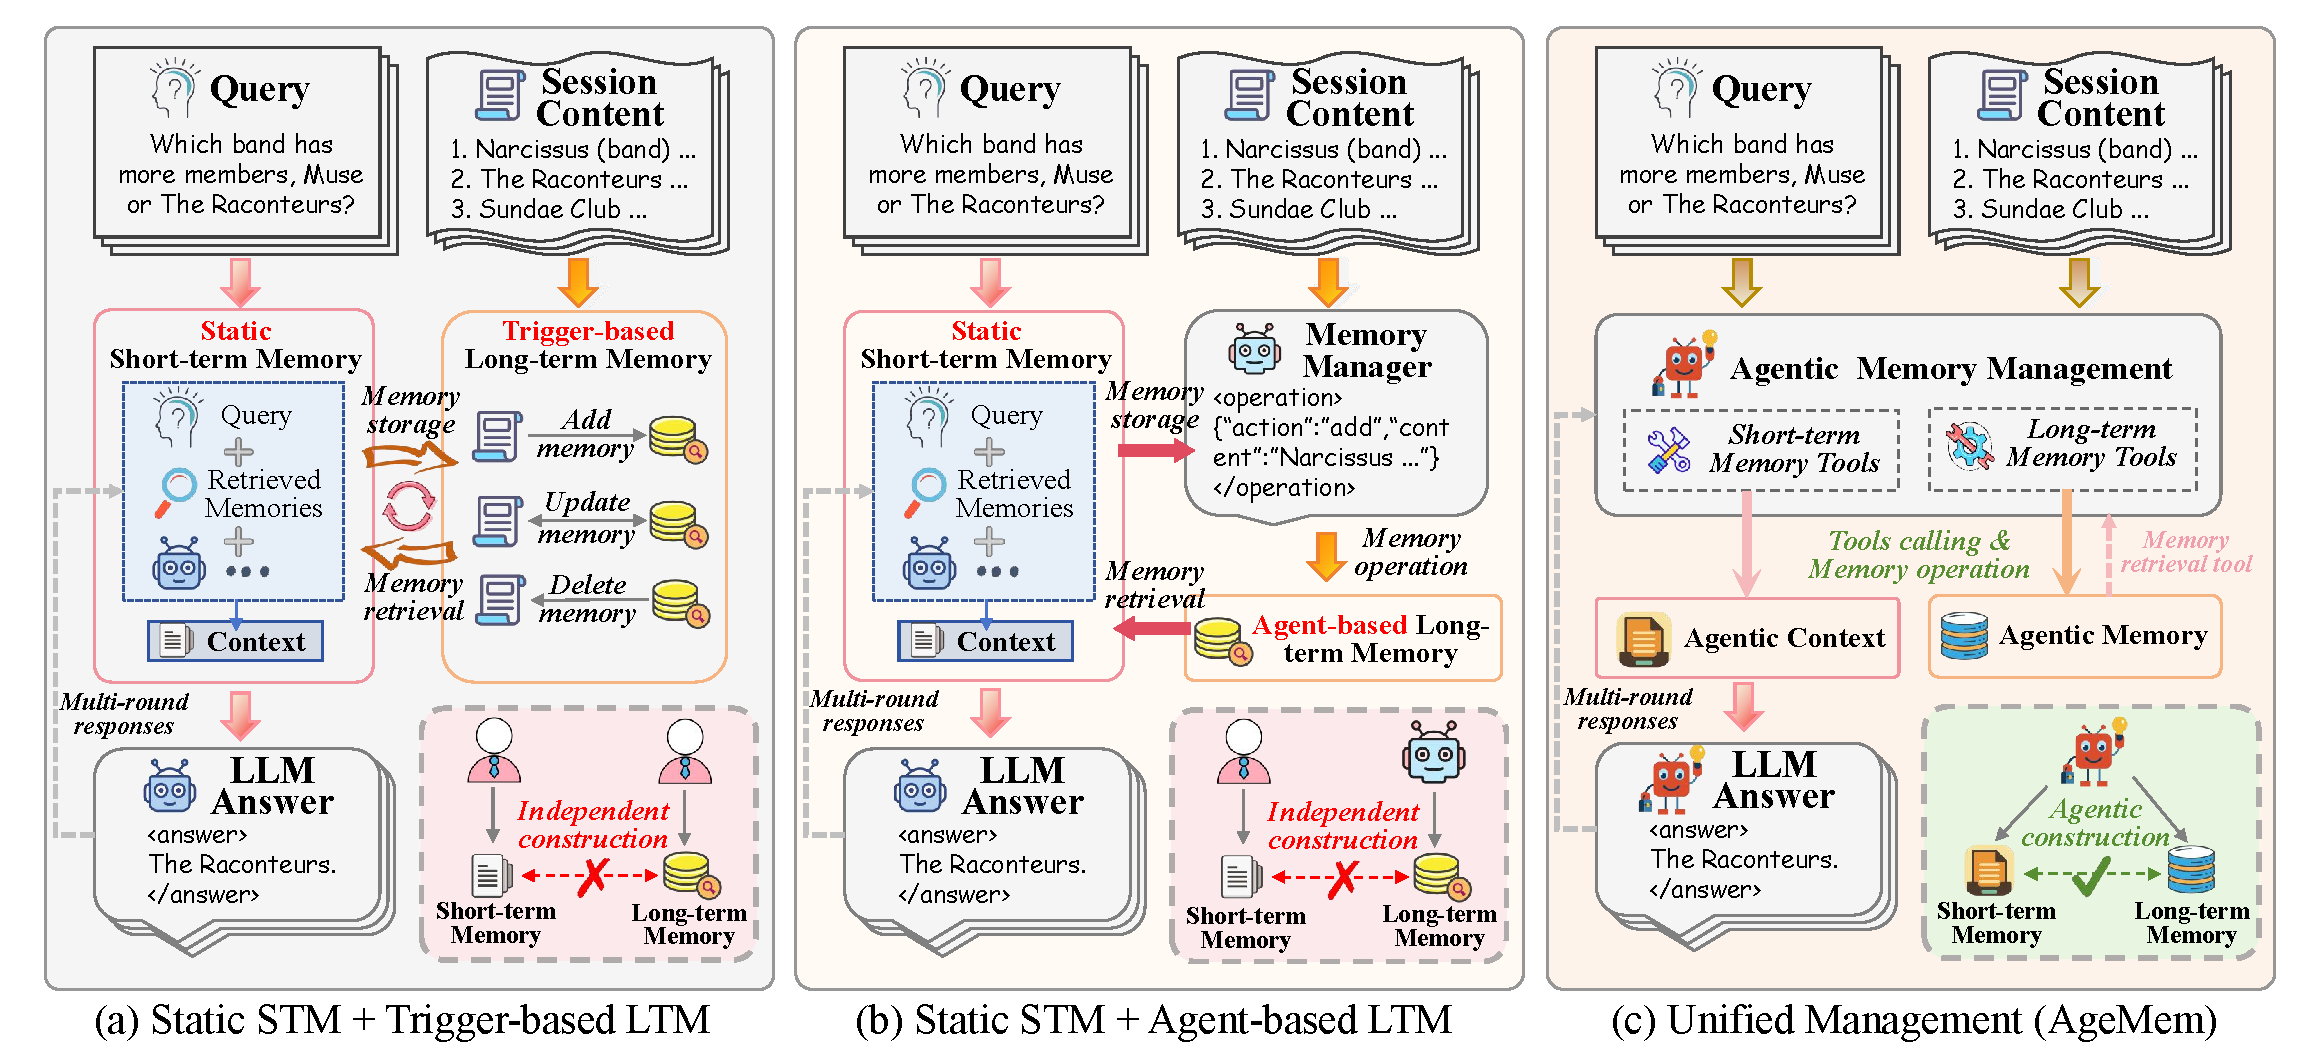
\includegraphics[width=\textwidth]{sections/pics/framework_new_addmode.pdf}
    \vspace{-7mm}
    \caption{Comparison between independent and unified memory management frameworks. (Left) Traditional framework with static STM and trigger-based LTM. (Middle) Independent framework with an additional Memory Manager controlling LTM in an agent-based manner, while STM remains static. (Right) The proposed AgeMem framework, where LTM and STM are \textbf{jointly} and \textbf{intelligently} managed via explicit tool-based operations.}
    \vspace{-3mm}
    \label{fig:framework}
\end{figure*}

However, existing research has predominantly treated LTM and STM as independent components. 
STM is commonly enhanced through retrieval-augmented generation (RAG)~\citep{pan2025memory}, such as in MainRAG~\citep{chang2025main} and ReSum~\citep{wu2025resum}, which expand usable context via external retrieval or periodic summarization.
Although effective in some tasks, these methods rely heavily on predefined schedules or heuristic rules, potentially resulting in overlooked infrequent but critical details as well as unnecessary noise~\citep{ma2025should, dong2025survey}.
In contrast, LTM management has progressed along separate lines, typically categorized into \emph{trigger-based}~\citep{kang2025memory, wang2025mirix, wang2025inducing, chhikara2025mem0} and \emph{agent-based}~\citep{yan2025memory, hu2025evaluating, xu2025mem} paradigms.
The former executes fixed memory operations at predefined moments, whereas the latter incorporates a specialized memory manager to determine what and how to store. 
Despite offering more flexibility, most approaches still depend on handcrafted rules or auxiliary expert models, limiting adaptability and increasing system complexity~\citep{xiong2025memory}.

As a consequence, LTM and STM are typically treated as \emph{separate and loosely coupled modules}. 
As illustrated in Figure~\ref{fig:framework}, existing architectures generally follow two patterns: 
(a) static STM with trigger-based LTM, or 
(b) static STM with agent-based LTM. 
In both settings, the two memory systems are optimized independently and later combined in an ad hoc way, leading to fragmented memory construction and suboptimal performance in long-horizon reasoning tasks.
Thus, unifying the management of LTM and STM remains a necessary yet largely unexplored challenge.

Nevertheless, achieving unified memory management poses three fundamental challenges. (\textbf{C1}) \textbf{Functional heterogeneity coordination:} LTM and STM serve distinct yet complementary purposes: LTM determines what to store, update, or discard, while STM governs what to retrieve, summarize, or remove from the active context~\citep{zhang2025survey}. The challenge lies in designing a unified mechanism that orchestrates their interplay synergistically. (\textbf{C2}) \textbf{Training paradigm mismatch:} Existing reinforcement learning (RL) frameworks adopt markedly different training strategies for the two memory types~\citep{ma2024coevolving}. LTM-focused training often leverages session-level information available prior to interaction, whereas STM training typically injects distractors to simulate long-horizon contexts~\citep{sun2024llm}. Moreover, standard RL assumes continuous trajectories with stable rewards, which conflicts with the inherently fragmented and discontinuous experiences produced by memory operations~\citep{wu2025resum}, making end-to-end optimization particularly challenging. (\textbf{C3}) \textbf{Practical deployment constraints:} Many agent systems rely on an auxiliary expert LLM for memory control, significantly increasing inference cost and training complexity. How to integrate unified memory management directly into an agent without dependence on external expert models remains an open problem.

To address these challenges, we propose \textit{Agentic Memory (AgeMem)}, a unified framework that jointly manages LTM and STM, illustrated in Figure~\ref{fig:framework} (right). 
Unlike prior designs that treat memory as an external component, AgeMem integrates both memory types directly into the agent’s decision-making process. Through a unified tool-based interface, the LLM autonomously invokes and executes memory operations for both LTM and STM. 
Furthermore, we design a three-stage progressive RL strategy: the model first acquires LTM storage capabilities, then learns STM context management, and finally coordinates both forms of memory under full task settings. 
To address the fragmented experience issue across training stages, we design a step-wise Group Relative Policy Optimization (GRPO)~\citep{shao2024deepseekmath}, which transforms cross-stage dependencies into learnable signals, thereby alleviating the challenges posed by sparse and discontinuous rewards in RL. We evaluate AgeMem on five long-context, reasoning-intensive benchmarks. Comprehensive results show that AgeMem consistently outperforms strong baselines, validating the effectiveness of unified memory management.

Our main contributions are as follows:
\begin{itemize}[leftmargin=*, topsep=0pt, itemsep=0pt, parsep=0pt]
\item We propose \textit{Agentic Memory (AgeMem)}, a unified \textbf{agentic memory framework} that enables LLM-based agents to autonomously decide \textbf{when}, \textbf{what}, and \textbf{how} to manage both long-term and short-term memory.
\item We develop a \textbf{three-stage progressive RL strategy} equipped with a step-wise GRPO mechanism, facilitating effective end-to-end learning of unified memory management behaviors.
\item We conduct \textbf{comprehensive evaluations} across multiple models and long-horizon benchmarks, demonstrating the robustness and effectiveness of AgeMem in complex agentic tasks.
\end{itemize}


